\chapter{引言}
\section{背景}
近年来,能源危机以及由于能源的不合理运用所带来的环境污染\cite{Goodenough2015Energy}等问题已经越来越成为制约着人类经济社会发展的关键因素。
在针对这一核心问题的诸多探索和尝试中,寻求一种可以足够安全地储存能量并能相对容易和高效地将储存的能量转换为电能的方式和器件尤为重要\cite{Feng2017Thermal}。同时,在方兴未艾的汽车电动化和新兴的自动驾驶等技术的发展浪潮中,汽车的能源储备系统正在经历着从化石能源到电化学能源\cite{Shan2016The,Tarascon2001Issues,Dunn2011Electrical}的广泛和深刻的变革。 而在这场变革中,锂离子电池系统由于有着高能量密度,使用寿命长乃至对环境相对友好的优点得到了广泛的应用\cite{Yoshio2003Spherical,Taberna2006High}并被赋予深厚的希望。 实际上,我们正在迅速接近车辆电动化的临界点,主要的汽车生产商都制定了雄心勃勃的各系列电动汽车的生产计划。 根据国际能源组织的统计,到2025年,全世界的电动汽车的保有量将达到一亿辆\cite{plan}。 巨大的市场和行业的迅速成长所带来的对车载电池的能量密度增长和对于电池成本降低的迫切需求,都带来了整个社会对于电动汽车安全性方面的担忧\cite{Zhu2018A}。\\
\indent考虑到每年电动汽车的巨额销量和迅速增长的保有量,可以预料到,这些车辆会不可避免地遭遇汽车碰撞事故,而在碰撞事故中,其电池系统会经历很多频繁的侵入或者冲击加载\cite{Xu2016Computational}。 同时,电池能量密度的提升和电动汽车对里程数的增加要求必然也会导致在相同的情况下电池受损造成的后果愈加严重。 实际上近几年,锂离子电池的故障导致的一些电动汽车的火灾和爆炸事件屡见报端\cite{volt,BYD,boeing,Tesla}(见图[\ref{fig:accident}]),造成了愈演愈烈的对于车载电池安全性的担忧。
\begin{figure}
\centering   
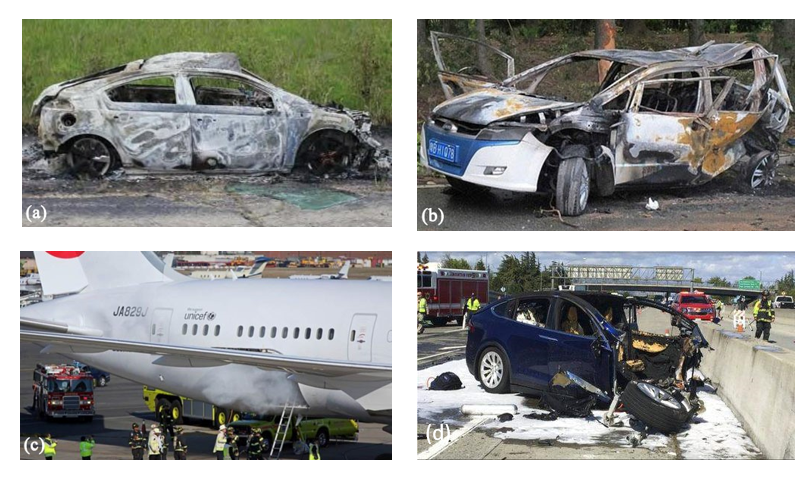
\includegraphics[width=\textwidth]{accident.png}
\caption{锂离子动力电池火灾:(a) Chevrolet Volt (b) BYD e6 (c) Boeing 787 (d) Tesla Model X } 
\label{fig:accident}
\end{figure}
\\
\indent 到目前为止,在所有会造成电池失效的因素如,制造缺陷、过充和过放\cite{Kermani2017Review}中,机械滥用是其中十分重要但是尚未得到充分研究和深刻理解的因素。 长期以来,对于锂离子电池的研究大多数都集中在对于其内部电化学过程的研究,对于其机械失效的研究十分稀少。而实际上,在碰撞事故中,电动汽车的车载电池包将有很大可能受到复杂外载从而产生变形,而这可能引起电池的内短路进一步发展成热失效从而引起诸如着火和爆炸等严重后果。 举例而言,内短路会由于机械外载造成的电池接头的外部保护失效从而导致正极和负极接触而产生。 由此可见,对于电池组分乃至结构单体到模组的力学性质和变形响应的定量探究和理解十分重要。\\
\indent 锂离子电池的力学失效特性和进一步所引发的热失效的整个过程有着多尺度,多物理场、非线性的特点,使得对于其的研究有很大的困难。一般而言,对于锂离子电池的力学失效特性的研究主要按照研究尺度和测试条件展开。 首先,最小的层次是晶体和颗粒层次,在这一层次往往可以研究电化学和力学行为的耦合特性,有着一系列的微观测试和模拟计算的方法。 在这一尺度,研究者对于电极体积的脱锂和嵌锂的变化,活性颗粒的变形和开裂,力学外载造成的电极材料性能衰退,内部应力分布乃至固体电解质膜的形成及其力学电学特性\cite{Behrou2017Multiscale,Behrou2017Numerical,Zhao2012Fracture,Zhao2010Fracture}进行了研究。 其次,相当多的研究对于电池的组成成分如电极、隔膜在不同力学外载下的力学响应\cite{Cannarella2014Mechanical,Zhang2016Li,Kalnaus2017Mechanical,Sheidaei2011Mechanical}进行了测试和建模。 另外还有对于电池的单体的诸多测试和力学建模的均质化模型和精细模型的研究\cite{Elham2012Calibration,Greve2012Mechanical,Sahraei2012Modeling,Sahraei2014Characterizing},乃至模组和系统层次的研究\cite{Ali2015Computational,Wang2017Progressive,Xia2014Damage,Kukreja2016Crash}。 
表\ref{tab:component}展示了对于锂离子电池的组分力学测试的研究和相关结果。
\begin{table}
    \centering
    \caption{重复单元组分及其力学性质}
    \label{tab:component}
    \begin{tabular}{ | c | p{1.8cm} | p{1.8cm} | p{0.5cm}|}
    \hline
    组分 & 材料 & 力学响应 & 参考文献 \\ \hline
    集流体 & 铝箔/铜箔 & 各向同性 应变硬化 塑性断裂 应变率响应 & \cite{Sahraei2016Microscale} \quad \quad  \cite{Sahraei2015Modelling} \quad \quad \cite{Greve2012Mechanical} \quad \quad \cite{Luo2015Fracture} \\
    涂层 & 石墨颗粒/活性物质颗粒 & 压力相关 & \cite{Dass} \\
    隔膜 & 多孔有机物 & 各向异性 粘弹塑性 温度相关  &  \cite{Huang2011Separator} \quad \quad \cite{Lee2014A} \quad \quad \cite{Zhang2016Deformation} \\ \hline
    \end{tabular}
\end{table}
\section{锂离子电池力学性质研究现状}
前文已经指出,在电动汽车的碰撞事故中,如果电池包产生结构损伤、分裂就有可能发生电池的热失控并引起火灾甚至爆炸。 为了对车载锂离子电池进行安全防护的研究和设计,需要对其力学外载响应和电化学-力学耦合响应有一个清晰的认识和理解,而这其中涉及了多尺度、多物理场的复杂问题(见图\ref{fig:zhu})。\\
\begin{figure}
\centering   
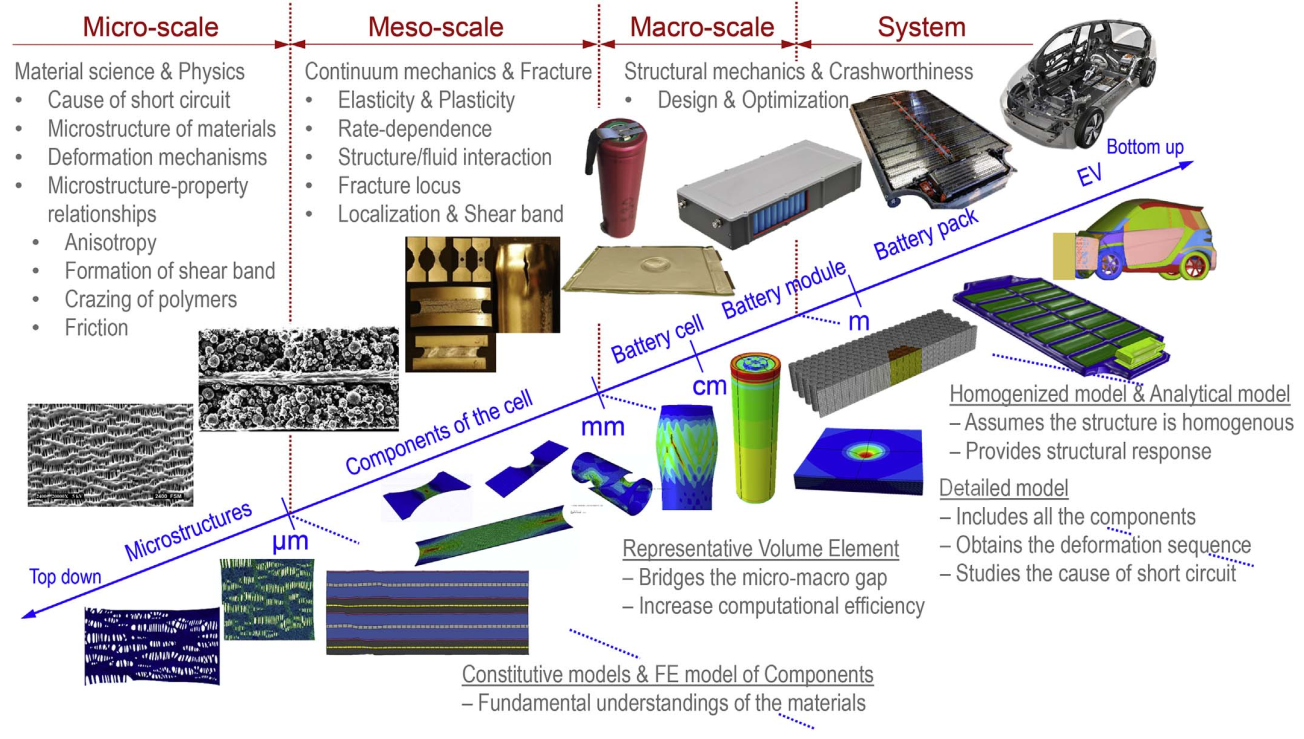
\includegraphics[width=\textwidth]{zhu.png}
\caption{锂离子电池力学性质研究涉及多个尺度和层面}
\label{fig:zhu}
\end{figure}
\indent 在介绍本文的研究内容之前,首先有必要对于锂离子电池的构成和组分进行简要介绍并对之前的对于组分力学性质的研究做一个归纳和总结。\\
\begin{figure}
\centering   
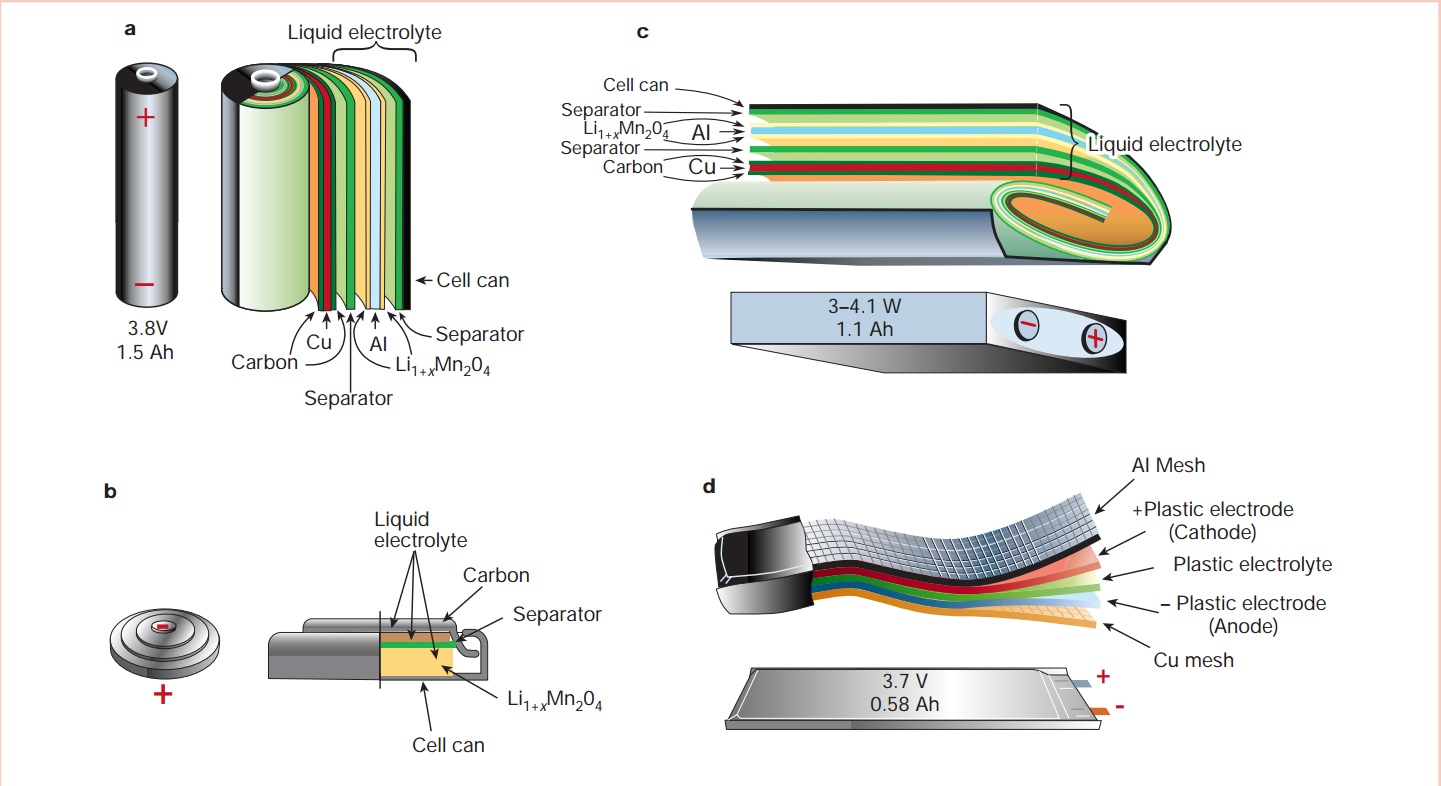
\includegraphics[width=\textwidth]{battery.png}
\caption{各种锂离子电池的形状和组成的示意图\cite{Tarascon2001Issues}:(a)圆柱形 (b)方形 (c)纽扣形 (d)软包形}
\label{fig:battery}
\end{figure}
\indent 锂离子电池作为一种典型的二次电池,其工作原理是依靠锂离子在电池的正极和负极的嵌入和脱嵌来传递电流。 其典型的类型按照形状来划分有圆柱型(如18650)、方形、纽扣形和软包形(图\ref{fig:battery})。 就微观和介观结构而言,商用车载锂离子电池通常采用多层电极堆叠的结构(见图(\ref{fig:structure}a)),其每一个重复单元由正极、负极和隔膜组成。 更细致而言,正极是由两侧涂布有活性物质层的铝箔组成,类似地,负极是由两侧涂布着石墨或者硅颗粒的铜箔组成。 这些成分都浸润在电解液中并被钢壳或者铝塑膜覆盖密封。 在电子显微镜下可以清晰分辨出正极和负极的三明治结构和隔膜的多孔结构(见图(\ref{fig:structure}b-d))。
\begin{figure}
\centering   
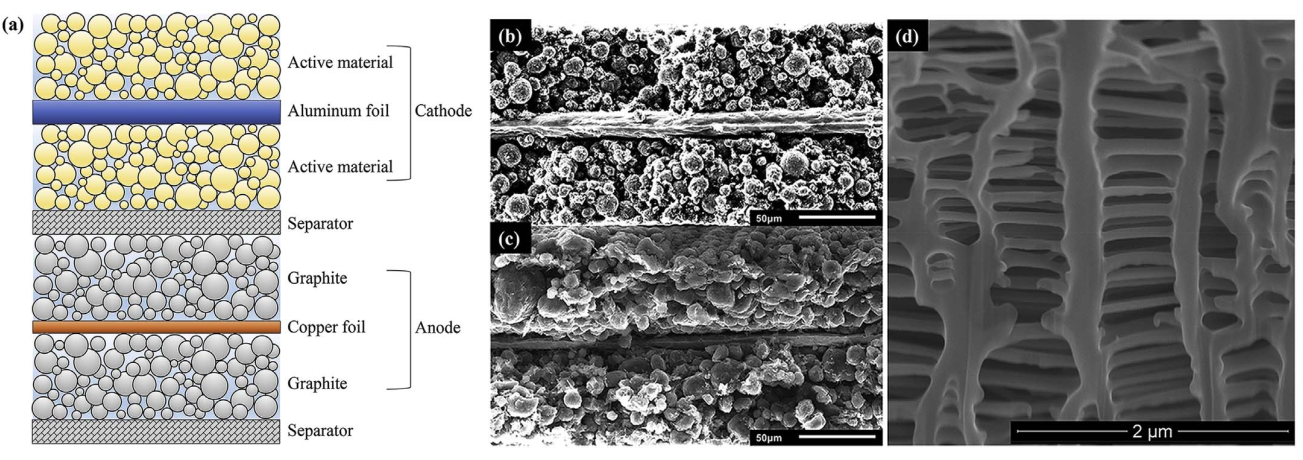
\includegraphics[width=\textwidth]{structure.png}
\caption{(a)锂离子电池的重复单元和组分的截面图 (b)正极 (c)负极 (d)隔膜}
\label{fig:structure}
\end{figure}
\section{研究目标}
对当前的电动汽车产业而言,如何在保证其安全性和可靠性的前提下设计出有着更高能量密度和更长寿命周期的电池至关重要。 为了实现这个目标,开展了大量关于电极活性材料的研究\cite{Cheng2011Functional,Park2015LiFeO2},然而,其中少有涉及到对于活性层和集流体的胶接强度的研究,而实际上保证足够的胶接强度无论对于充放电循环的实现和电池寿命的保证还是对于安全防护都至关重要\cite{Chen2013Unveiling}。\\
\indent 一方面电池周期性的充放电循环会产生交替的内应力,可能会导致活性物质内部裂纹的产生甚至活性层和集流体的分层这些不可逆的变化,从而可能导致电池容量的减小和循环次数的减少\cite{Vetter2005Ageing}。 研究表明,对于硅-锡电池系统(其在锂离子脱嵌和嵌入过程中的体积变化可以高达250\%)而言,即使其活性颗粒在体积膨胀和收缩的过程中不发生断裂,依然会发生活性颗粒之前的电接触条件变差(接触面减小或者脱离接触)导致容量减小\cite{Chen2003A,Chen2003Large}。 所以,为了保证一个良好的电池生命周期,在活性物质和集流体之间维持良好的连接条件显得至关重要。
\begin{figure}
\centering   
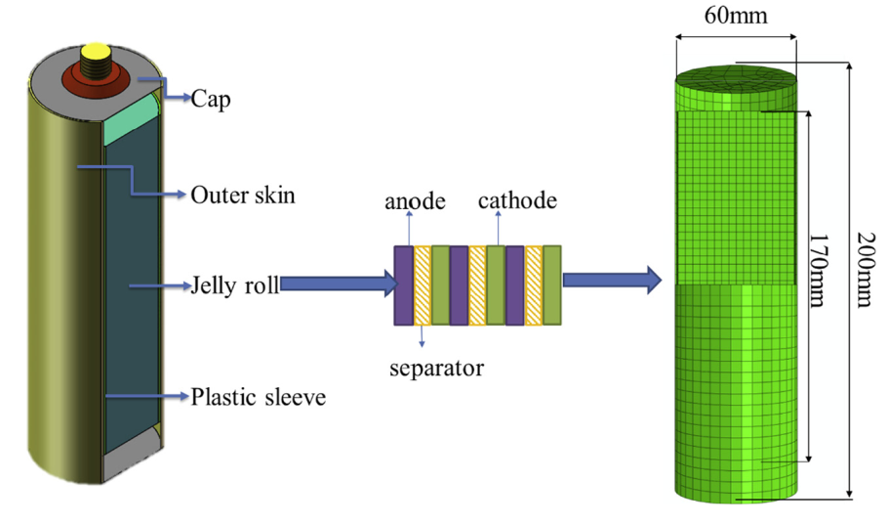
\includegraphics[width=0.8\textwidth]{homo.png}
\caption{HP 602030电池的均质化有限元模型}
\label{fig:homo}
\end{figure}\\
\indent 另一方面,为了准确的表征电动汽车的碰撞工况和车载电池的碰撞响应,需要建立准确的有限元模型。 起初建立的模型大多是均质化的有限元模型,在这些模型中,整个电池单体被看做是同种材料进行建模(见图(\ref{fig:homo})),但是实际的碰撞工况往往涉及大变形和多种形式的动态加载,使得简单的均质化建模难以准确预测电池在碰撞事故中的失效行为\cite{Luo2018Adhesion}。 随着对于电池组分材料力学行为的测试和表征,基于这些数据建立精细化的有限元模型有望相对准确地分析和预测电池的碰撞失效演变行为\cite{Lu2013A}。 而在电池组分水平,其多层结构中的界面力学特性,如活性层粘接强度,尚未得到充分的研究,而在力学有限元建模中界面力学特性会明显影响电池在外部加载下的局部和总体的力学响应。\\
\indent 同时,前文也指出,对于电池力学性质的研究往往很少考虑电化学因素的影响,而对于锂离子电化学性能的研究却也很少包括对于力学特性的表征。 而本文所关注的锂离子电池活性层-集流体界面强度的研究必然包括着对于锂离子扩散过程的考量,也就意味着如果想要建立一个全面的模型必须要同时对于力学和电化学因素进行综合考虑。\\
\indent 总结而言,对于锂离子电池界面力学性质的测试和表征是一项有意义和有挑战的工作,尤其是探究其在混合加载和动态加载等接近实际工况下的力学响应。 本研究的目的在于直接测定集流体和活性层在混合力学加载下的的粘接强度,从而为精细化的力学建模提供模型参数的支持以及为预测界面脱层失效乃至电池失效响应提供实验支持。另外本研究将利用分子模拟的手段从微观层面对于颗粒在锂离子脱嵌和嵌入过程这一锂离子电池循环周期中关键的电化学过程中的颗粒的力学特性乃至其断裂特征进行研究,从而补充和佐证界面力学测试实验,并为进一步的耦合研究提供基础。
\section{文章架构}
本文第2章将探讨界面力学实验方案的设计,首先将介绍现有研究方法的特点和不足,进而对于胶接作用中断裂失效的可能模式进行了分类,提出一种获得给定的活性层-集流体界面脱层失效模态的实验方法。 另外将介绍实验的准备工作,包括对于实验方法的验证分析以及对于在后续分析中所会用到的断裂准则和内聚力模型进行了介绍。 \\
\indent
第3章在第2章的基础上讨论和分析了电池正极和负极的静态和动态实验的测试结果,并给出了包括了电化学影响的颗粒-壳体模型来在微观层面进行力学表征。 \\
\indent 第4章首先利用第一性原理计算的方法计算出了$Li$离子在$LiFePO_4$晶体中沿着两个不同方向进行扩散的能垒和反应活性并得到了主要扩散方向上进行扩散时的扩散路径, 接下来基于此同样采用第一性原理计算的方法对于其在$Li$离子扩散过程中晶体的弹性常数及相应力学参数的变化进行了研究,同时也讨论了其力学各向异性;最后利用分子动力学计算的方法对于$Li$离子扩散前后的$LiFePO_4$晶体进行应变加载,并在模拟中成功观察到了其断裂失效行为。 \\
\indent
第5章对于全文结果进行了总结分析,并提出了对接下来可能进行的工作的展望。